\documentclass[journal,12pt,onecolumn]{IEEEtran}
\usepackage{cite}
\usepackage{amsmath,amssymb,amsfonts,amsthm}
\usepackage{algorithmic}
\usepackage{graphicx}
\graphicspath{{./figs/}}
\usepackage{textcomp}
\usepackage{xcolor}
\usepackage{txfonts}
\usepackage{listings}
\usepackage{enumitem}
\usepackage{mathtools}
\usepackage{gensymb}
\usepackage{comment}
\usepackage{caption}
\usepackage[breaklinks=true]{hyperref}
\usepackage{tkz-euclide} 
\usepackage{listings}
\usepackage{gvv}                                            
\usepackage{xparse}
\usepackage{color}                                            
\usepackage{array}                                            
\usepackage{longtable}                                       
\usepackage{calc}                                             
\usepackage{multirow}
\usepackage{multicol}
\usepackage{hhline}                                           
\usepackage{ifthen}                                           
\usepackage{lscape}
\usepackage{tabularx}
\usepackage{array}
\usepackage{float}
\usepackage[margin=1in]{geometry}
\usepackage{fancyhdr}
\usepackage{chemfig}
\usepackage{multicol}
\usepackage{amsmath}
\usepackage{enumitem}
\usepackage{array}
\usepackage{titlesec}
\usepackage{tabularx}
\usepackage{amssymb}
\usepackage{extarrows}
\usepackage{chemarr}
\usepackage[utf8]{inputenc}
\usepackage{chemmacros}
\usepackage{graphicx}
\chemsetup{modules={reactions}}

\pagestyle{fancy}
\fancyhf{}
\fancyhead[L]{\textit{2012}}
\fancyhead[R]{\textbf{LIFE SCIENCES--XL}}
\renewcommand{\headrulewidth}{0.4pt}

\begin{document}

% ==============================
\section*{\centering GA : GENERAL APTITUDE (Compulsory)}

\noindent \textbf{1 -- 5 carry one mark each.}
\begin{enumerate}[label=\arabic*.]
\item If $(1.001)^{1259} = 3.52$ and $(1.001)^{2062} = 7.85$, then $(1.001)^{3321} =$ 
\begin{multicols}{4}
\begin{enumerate}[label=(\Alph*)]
\item 2.23
\item 4.33
\item 11.37
\item 27.64
\end{enumerate}
\end{multicols}

\item One of the parts (A, B, C, D) in the sentence given below contains an ERROR. Which one of the following is \textbf{INCORRECT}?

\textbf{I requested that he should be given the driving test today instead of tomorrow.}

\begin{enumerate}[label=(\Alph*)]
\item requested that
\item should be given
\item the driving test
\item instead of tomorrow
\end{enumerate}

\item Which one of the following options is the closest in meaning to the word given below?\\
\textbf{Latitude}
\begin{multicols}{4}
\begin{enumerate}[label=(\Alph*)]
\item Eligibility
\item Freedom
\item Coercion
\item Meticulousness
\end{enumerate}
\end{multicols}

\item Choose the most appropriate word from the options given below to complete the following sentence:\\
\textbf{Given the seriousness of the situation that he had to face, his \_\_\_\_ was impressive.}
\begin{multicols}{4}
\begin{enumerate}[label=(\Alph*)]
\item beggary
\item nomenclature
\item jealousy
\item nonchalance
\end{enumerate}
\end{multicols}

\item Choose the most appropriate alternative from the options given below to complete the following sentence:\\
\textbf{If the tired soldier wanted to lie down, he \_\_\_\_ the mattress out on the balcony.}
\begin{multicols}{2}
\begin{enumerate}[label=(\Alph*)]
\item should take
\item shall take
\item should have taken
\item will have taken
\end{enumerate}
\end{multicols}


\noindent \textbf{6 -- 10 carry two marks each.}

\item \textbf{One of the legacies of the Roman legions was discipline. In the legions, military law prevailed and discipline was brutal. Discipline on the battlefield kept units obedient, intact and fighting, even when the odds and conditions were against them.}

Which one of the following statements best sums up the meaning of the above passage?
\begin{enumerate}[label=(\Alph*)]
\item Thorough regimentation was the main reason for the efficiency of the Roman legions even in adverse circumstances.
\item The legions were treated inhumanly as if the men were animals.
\item Discipline was the armies’ inheritance from their seniors.
\item The harsh discipline to which the legions were subjected to led to the odds and conditions being against them.
\end{enumerate}

\item A and B are friends. They decide to meet between 1 PM and 2 PM on a given day. There is a condition that whoever arrives first will not wait for the other for more than 15 minutes. The probability that they will meet on that day is
\begin{multicols}{2}
\begin{enumerate}[label=(\Alph*)]
\item $1/4$
\item $1/16$
\item $7/16$
\item $9/16$
\end{enumerate}
\end{multicols}

\item The data given in the following table summarizes the monthly budget of an average household.\\[2pt]
\begin{tabular}{|l|c|}
\hline
\textbf{Category} & \textbf{Amount (Rs.)} \\
\hline
Food & 4,000 \\
Clothing & 1,200 \\
Rent & 2,000 \\
Savings & 1,500 \\
Other expenses & 1,800 \\
\hline
\end{tabular}\\[2pt]
The approximate percentage of the monthly budget \textbf{NOT} spent on savings is
\begin{multicols}{2}
\begin{enumerate}[label=(\Alph*)]
\item 10\%
\item 14\%
\item 81\%
\item 86\%
\end{enumerate}
\end{multicols}

\item There are eight bags of rice looking alike, seven of which have equal weight and one is slightly heavier. The weighing balance is of unlimited capacity. Using this balance, the minimum number of weighings required to identify the heavier bag is
\begin{multicols}{2}
\begin{enumerate}[label=(\Alph*)]
\item 2
\item 3
\item 4
\item 8
\end{enumerate}
\end{multicols}

\item Raju has 14 currency notes in his pocket consisting of only Rs. 20 notes and Rs. 10 notes. The total money value of the notes is Rs. 230. The number of Rs. 10 notes that Raju has is
\begin{multicols}{2}
\begin{enumerate}[label=(\Alph*)]
\item 5
\item 6
\item 9
\item 10
\end{enumerate}
\end{multicols}
\end{enumerate}

\newpage
\section*{\centering H : CHEMISTRY (Compulsory)}

\noindent \textbf{1 -- 5 carry one mark each.}
\begin{enumerate}[label=\arabic*.]
\item Among the following, the most reactive diene in the Diels-Alder reaction is

\begin{enumerate}[label=(\Alph*)]
\item \scalebox{0.7}{\chemfig{=*6(-=----)}}
\item \scalebox{0.7}{\chemfig{(=[:150]-[:90]=[:30])}}
\item \scalebox{0.7}{\chemfig{*5(=-=-O-)}}
\item \scalebox{0.7}{\chemfig{*5(=-=--)}}
\end{enumerate}


\item The molecule that does \textbf{NOT} absorb the microwave radiation is
\begin{multicols}{2}
\begin{enumerate}[label=(\Alph*)]
\item CO$_2$
\item H$_2$O
\item CO
\item NO
\end{enumerate}
\end{multicols}

\item The hybridization of atomic orbitals of sulphur in SF$_4$ is
\begin{multicols}{2}
\begin{enumerate}[label=(\Alph*)]
\item dsp$^2$
\item sp$^3$d$^2$
\item sp$^3$d
\item sp$^3$
\end{enumerate}
\end{multicols}

\item The ionic size of Na$^+$, F$^-$, Mg$^{2+}$ and Al$^{3+}$ varies as
\begin{multicols}{2}
\begin{enumerate}[label=(\Alph*)]
\item Al$^{3+} >$ Mg$^{2+} >$ Na$^+ >$ F$^-$
\item F$^- >$ Na$^+ >$ Mg$^{2+} >$ Al$^{3+}$
\item Al$^{3+} >$ Mg$^{2+} >$ F$^- >$ Na$^+$
\item Na$^+ >$ F$^- >$ Mg$^{2+} >$ Al$^{3+}$
\end{enumerate}
\end{multicols}

\item The non-aromatic compound/ion is

\item \begin{figure}[H]
    \centering
    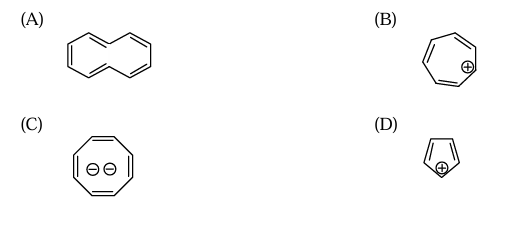
\includegraphics[width=0.7\columnwidth]{FIG/H-5.png}
    \caption*{}
    \label{fig:H-5}
\end{figure}

\noindent \textbf{6 -- 15 carry two marks each.}

\item As predicted by MO theory, the bond order and magnetic nature of NO$^+$ are
\begin{multicols}{2}
\begin{enumerate}[label=(\Alph*)]
\item three and paramagnetic
\item two and diamagnetic
\item two and paramagnetic
\item three and diamagnetic
\end{enumerate}
\end{multicols}

\item The value of ionic product of water changes with temperature. It is $1 \times 10^{-14}$ at 25$^\circ$C and $1 \times 10^{-13}$ at 60$^\circ$C. The \textbf{CORRECT} statement with respect to $\Delta H$ and $\Delta S$ is
\begin{multicols}{2}
\begin{enumerate}[label=(\Alph*)]
\item $\Delta H$ is negative and $\Delta S$ is negative
\item $\Delta H$ is positive and $\Delta S$ is zero
\item $\Delta H$ is positive and $\Delta S$ is negative
\item $\Delta H$ is negative and $\Delta S$ is positive
\end{enumerate}
\end{multicols}

\item 10 micrograms of the enzyme carbonic anhydrase (molecular weight = 30,000 g/mole) removes 300 milligrams of carbon dioxide per minute from the cells. The turnover number of the enzyme is
\begin{multicols}{2}
\begin{enumerate}[label=(\Alph*)]
\item $20$ min$^{-1}$
\item $2 \times 10^{7}$ min$^{-1}$
\item $2 \times 10^{10}$ min$^{-1}$
\item $7.2 \times 10^{10}$ min$^{-1}$
\end{enumerate}
\end{multicols}

\item The iodide which reacts most slowly with cyanide ion as a nucleophile in a SN2 reaction is

\begin{multicols}{2}
\begin{enumerate}[label=(\Alph*)]
\item CH$_3$CH$_2$CH$_2$CH$_2$I
\item \scalebox{0.7}{\chemfig{ICH_2-*6(-=-=-=)}}
\item \scalebox{0.7}{\chemfig{I-*3(---)}}
\item (CH$_3$)$_2$CH–I
\end{enumerate}
\end{multicols}

\item The value of $K_a$ of acetic acid is $1.7 \times 10^{-5}$ mol/dm$^3$. The pH of a buffer solution prepared by mixing 100 ml of 0.1 M acetic acid with a solution of 100 ml of 0.2 M sodium acetate is
\begin{multicols}{2}
\begin{enumerate}[label=(\Alph*)]
\item 4.1
\item 4.5
\item 5.1
\item 5.5
\end{enumerate}
\end{multicols}

\item The value of standard half cell potential of Cu$^{2+}$, Cu couple ($E^0_{Cu^{2+}, Cu}$) is 0.34 V. A wire of pure copper is immersed into a solution of copper nitrate. If the measured cell potential against standard hydrogen electrode at 298 K is 0.24 V, the molar concentration of copper nitrate is (Assume activity of Cu$^{2+}$ = [Cu$^{2+}$].)
\begin{multicols}{2}
\begin{enumerate}[label=(\Alph*)]
\item $4.1 \times 10^{-4}$ M
\item $2.0 \times 10^{-2}$ M
\item $3.4 \times 10^{-2}$ M
\item $1.8 \times 10^{-1}$ M
\end{enumerate}
\end{multicols}

\noindent\textbf{Common Data Questions}

\noindent\textbf{Common Data for Questions 12 and 13:}

$[$FeCl$_4]^{2-}$ (I), $[$CoCl$_4]^{2-}$ (II) and $[$NiCl$_4]^{2-}$ (III) are paramagnetic tetrahedral complexes.

\item The order of values of crystal field stabilization energy is
\begin{multicols}{2}
\begin{enumerate}[label=(\Alph*)]
\item I $>$ III $>$ II
\item III $>$ I $>$ II
\item I $>$ II $>$ III
\item II $>$ III $>$ I
\end{enumerate}
\end{multicols}

\item The order of values of spin only magnetic moment is
\begin{multicols}{2}
\begin{enumerate}[label=(\Alph*)]
\item III $>$ II $>$ I
\item III $>$ I $>$ II
\item II $>$ I $>$ III
\item I $>$ II $>$ III
\end{enumerate}
\end{multicols}

\noindent\textbf{Linked Answer Questions 14, 15}

\noindent\textbf{Statement for Linked Answer Questions 14 and 15:}

Bromine water is decolourised upon reaction with (E)-3-hexene.

\item It is due to
\begin{multicols}{2}
\begin{enumerate}[label=(\Alph*)]
\item electrophilic addition of bromine to C=C
\item nucleophilic addition of bromine to C=C
\item electrophilic allylic bromination
\item nucleophilic allylic bromination
\end{enumerate}
\end{multicols}

\item The structure of the product obtained is

\begin{figure}[H]
    \centering
    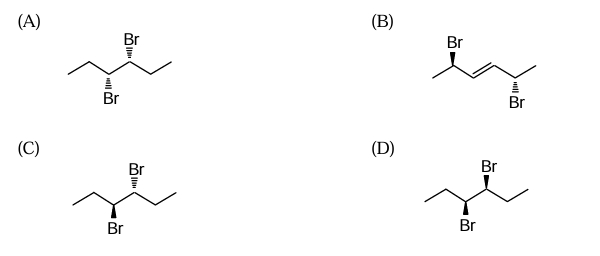
\includegraphics[width=0.7\columnwidth]{FIG/H-15.png}
    \caption*{}
    \label{fig:H-15}
\end{figure}
\end{enumerate}

\begin{center}
\textbf{END OF SECTION - H}
\end{center}
\newpage
\section*{\centering I : BIOCHEMISTRY}

\noindent \textbf{ 1 --  10 carry one mark each.}
\begin{enumerate}[label=\arabic*.]
\item Four proteins (P1, P2, P3 and P4) have 17, 10, 21 and 14 percent hydrophobic amino-acids respectively. The order of precipitation of these proteins using ammonium sulphate will be
\begin{multicols}{4}
\begin{enumerate}[label=(\Alph*)]
\item P3, P1, P4, P2
\item P3, P1, P2, P4
\item P2, P4, P3, P1
\item P2, P4, P1, P3
\end{enumerate}
\end{multicols}

\item Which one of the following pairs of amino-acids in the protein has high propensity to take up the $\alpha$-helix conformation?
\begin{multicols}{4}
\begin{enumerate}[label=(\Alph*)]
\item Gly-Asp
\item Pro-His
\item Gly-Pro
\item Ala-Arg
\end{enumerate}
\end{multicols}

\item Which one of the following closely defines `Molten Globule’ state of a protein?
\begin{enumerate}[label=(\Alph*)]
\item State with high degree of secondary structure and loss of tertiary structure
\item State with complete loss of secondary structure
\item Completely unfolded state
\item Loss of quaternary structure
\end{enumerate}

\item Which one of the following amino-acids has highest fluorescence quantum yield ($\Phi$) in aqueous solution?
\begin{multicols}{4}
\begin{enumerate}[label=(\Alph*)]
\item Tyrosine 
\item Tryptophan 
\item Phenylalanine 
\item Histidine
\end{enumerate}
\end{multicols}

\item Which one of the following compounds does NOT block electron transport?
\begin{multicols}{4}
\begin{enumerate}[label=(\Alph*)]
\item Cyanide
\item Rotenone
\item Oligomycin
\item Antimycin A
\end{enumerate}
\end{multicols}

\item The pair of amino-acids which does NOT undergo post-translational modification is
\begin{multicols}{4}
\begin{enumerate}[label=(\Alph*)]
\item Asn-His
\item Tyr-Ser
\item Asn-Ser
\item Ala-Gly
\end{enumerate}
\end{multicols}

\item Match the hormones in Group I with their metabolic precursor in Group II
\begin{center}
\begin{tabular}{p{7cm} p{8cm}}
\textbf{Group I} & \textbf{Group II} 
P. 17-$\beta$ estradiol & 1. Arachidonic acid 
 Thromboxane A$_2$   & 2. Tyrosine 
R. Epinephrine         & 3. $\beta$-carotene 
S. Retinoic acid       & 4. Cholesterol 
\end{tabular}
\end{center}
\begin{multicols}{2}
\begin{enumerate}[label=(\Alph*)]
\item P-4, Q-2, R-3, S-1
\item P-1, Q-3, R-2, S-4
\item P-4, Q-1, R-2, S-3
\item P-1, Q-2, R-4, S-3
\end{enumerate}
\end{multicols}

\item Upon stimulation of a eukaryotic cell, the intracellular calcium (Ca$^{2+}$) is released from
\begin{multicols}{4}
\begin{enumerate}[label=(\Alph*)]
\item Endoplasmic reticulum
\item Nucleus
\item Peroxisome
\item Mitochondria
\end{enumerate}
\end{multicols}

\item Leguminous plants maintain a very low concentration of free oxygen in their root nodules because
\begin{enumerate}[label=(\Alph*)]
\item the nitrogen fixing bacteria living in the root nodules are anaerobic
\item of binding of oxygen to leghemoglobin
\item reductase enzyme of the nitrogenase complex helps in removal of O$_2$
\item nitrogenase enzyme of the nitrogenase complex helps in removal of O$_2$
\end{enumerate}

\item The membrane of mature B cells have
\begin{multicols}{2}
\begin{enumerate}[label=(\Alph*)]
\item both IgG and IgM
\item both IgG and IgD
\item both IgM and IgE
\item both IgM and IgD
\end{enumerate}
\end{multicols}

\noindent \textbf{ 11 --  20 carry two marks each.}
\item An amino-acid has one proton donating group in the side chain (R). The p$K_{COOH}$, p$K_{NH2}$ and p$K_R$
values for this amino-acid are 2.19, 9.67 and 4.25, respectively. Which one of the following statements about this amino-acid is CORRECT?
\begin{enumerate}[label=(\Alph*)]
\item Majority of the molecules will have a net charge of -1 at pH of 7.0
\item Majority of the molecules will have a net charge of 0 at pH of 4.25
\item All the molecules will have a deprotonated R group at pH of 3.22
\item During titration with a strong base, deprotonation will start with the R group
\end{enumerate}

\item Which one of the following bacterial toxins does NOT have ADP-ribosyl transferase activity?
\begin{multicols}{2}
\begin{enumerate}[label=(\Alph*)]
\item Pertussis toxin
\item Diphtheria toxin
\item Pseudomonas Exotoxin A
\item S. aureus $\alpha$-toxin
\end{enumerate}
\end{multicols}

\item The CORRECT pair of amino-acid sequence and the corresponding target organelle is
\begin{multicols}{2}
\begin{enumerate}[label=(\Alph*)]
\item KDEL - Golgi
\item K-K/R-X-K/R - Lysosome
\item SKL - Peroxisome
\item NPVY - Endoplasmic reticulum
\end{enumerate}
\end{multicols}

\item $\beta$-oxidation of a 16 carbon fatty acid and a 17 carbon fatty acid leads to formation of
\begin{enumerate}[label=(\Alph*)]
\item (8 Acetyl CoA) and (8 Acetyl CoA + CO$_2$), respectively
\item (5 Propionyl CoA + 1 CO$_2$) and (5 Propionyl CoA + 1 Acetyl CoA), respectively
\item (5 Propionyl CoA + 1 CO$_2$) and (5 Propionyl CoA + 2 CO$_2$), respectively
\item (8 Acetyl CoA) and (7 Acetyl CoA + 1 Propionyl CoA), respectively
\end{enumerate}


\item Pick the correctly matched pairs.
\begin{enumerate}[label=\Alph*. ,start=16]
\item Immature B cells — Terminal deoxynucleotidyl transferase
\item Activated B cells — Class switching
\item Pre B cells       — Surrogate light chain
\item Mature B cells   — Recombination activating gene 1
\end{enumerate}
\begin{multicols}{4}
\begin{enumerate}[label=(\Alph*)]
\item P and R
\item Q and R
\item Q and S
\item Q and P
\end{enumerate}
\end{multicols}

\item The actual free energy change of a given biochemical reaction carried out under standard conditions with 1 M initial concentration of each of the reactants and products will be
\begin{enumerate}[label=(\Alph*)]
\item equal to zero
\item equal to standard free energy change for the reaction
\item less than the standard free energy change for the reaction
\item greater than the standard free energy change for the reaction
\end{enumerate}

\item Match the enzymes in Group I with their corresponding activity in Group II

\begin{center}
\begin{tabular}{p{5cm} p{8cm}}
\textbf{Group I} & \textbf{Group II} \\
P. Flippase      & 1. Catalyzes the movement of any phospholipid across the lipid bilayer down its concentration gradient\\
 Floppase      & 2. Catalyzes the translocation of amino-phospholipids from the extracellular to the inner leaflet\\
R. Lipase        & 3. Catalyzes the translocation of membrane phospholipids from cytosolic to extracellular leaflet\\
S. Scramblase    & 4. Degradation of phospholipids from the lipid bilayer including inner and outer leaflets\\
\end{tabular}
\end{center}
\begin{multicols}{2}
\begin{enumerate}[label=(\Alph*)]
\item P-2, Q-3, R-4, S-1
\item P-1, Q-2, R-3, S-4
\item P-4, Q-1, R-2, S-3
\item P-3, Q-2, R-4, S-1
\end{enumerate}
\end{multicols}

\item Match the antibiotics in Group I with their mechanism of action in Group II

\begin{center}
\begin{tabular}{p{5cm} p{8cm}}
\textbf{Group I} & \textbf{Group II}\\
P. Tetracyclines & 1. Inhibits bacterial protein synthesis by blocking peptidyl transfer\\
 Chloramphenicol & 2. Inhibits protein synthesis by blocking the A-site on the ribosome\\
R. Cycloheximide & 3. Misreads genetic code and inhibits initiation of protein synthesis\\
S. Streptomycin & 4. Inhibits protein synthesis by blocking peptidyl transferase on 80S ribosome\\
\end{tabular}
\end{center}
\begin{multicols}{2}
\begin{enumerate}[label=(\Alph*)]
\item P-2, Q-1, R-3, S-4
\item P-2, Q-1, R-4, S-3
\item P-4, Q-3, R-1, S-2
\item P-3, Q-4, R-2, S-1
\end{enumerate}
\end{multicols}

% For graphical/figure question 19, use an image placeholder
\item The kinetics of an enzyme in the presence (+I) or absence (–I) of a reversible inhibitor is described in the following graph.

\begin{figure}[H]
    \centering
    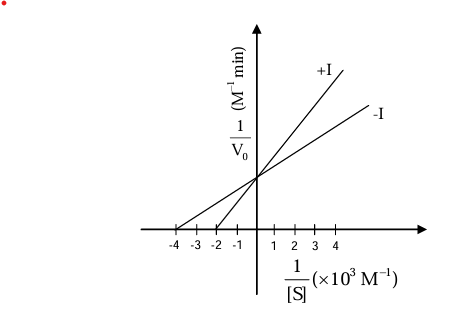
\includegraphics[width=0.7\columnwidth]{FIG/I-19.png}
    \caption*{}
    \label{fig:I-19}
\end{figure}

If concentration of the reversible inhibitor in +I experiment was equal to $3.0 \times 10^{-3}$ M, then the dissociation constant for the enzyme-inhibitor complex is\\

\begin{multicols}{2}
\begin{enumerate}[label=(\Alph*)]
\item $1 \times 10^{-3}$ M
\item $2 \times 10^{-3}$ M
\item $3 \times 10^{-3}$ M
\item $4 \times 10^{-3}$ M
\end{enumerate}
\end{multicols}

% Another graphical/figure question 20
\item The figure below is a schematic of a linear double stranded DNA containing the indicated restriction sites. The DNA was completely digested with PvuII and EcoRI. The products were purified and added to an appropriately buffered reaction mixture containing dNTP mix, $\alpha$-$^{32}$P dATP, and Klenow fragment of E. coli DNA polymerase I. The Klenow reaction products were analyzed by gel electrophoresis and autoradiography. Which of the following products depicts the expected result?\\
\begin{figure}[H]
    \centering
    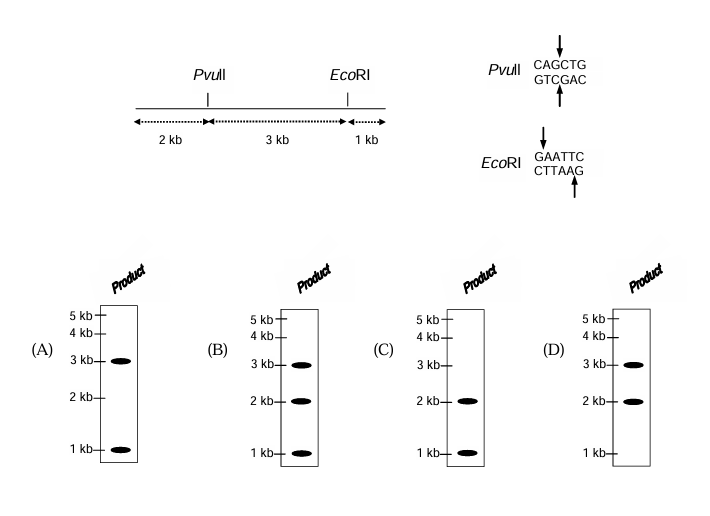
\includegraphics[width=0.7\columnwidth]{FIG/I-20.png}
    \caption*{}
    \label{fig:I-20}
\end{figure}


\end{enumerate}

\begin{center}
\textbf{END OF SECTION - I}
\end{center}
\newpage
\section*{\centering J : BOTANY}

\noindent \textbf{ 1 --  10 carry one mark each.}
\begin{enumerate}[label=\arabic*.]
\item The swollen base of a petiole is known as
\begin{multicols}{4}
\begin{enumerate}[label=(\Alph*)]
\item Ligule
\item Hastule
\item Pulvinus
\item Stipule
\end{enumerate}
\end{multicols}

\item An estimate of phylogenetic relationships among the taxa is commonly represented in the form of a
\begin{multicols}{4}
\begin{enumerate}[label=(\Alph*)]
\item Cladogram
\item Idiogram
\item Phenogram
\item Dendrogram
\end{enumerate}
\end{multicols}

\item Parenchyma cells associated with sieve tube members are called
\begin{multicols}{2}
\begin{enumerate}[label=(\Alph*)]
\item Albuminous cells
\item Companion cells
\item Bulliform cells
\item Subsidiary cells
\end{enumerate}
\end{multicols}

\item Cytoplasmic male sterility via the chloroplast genome can be induced by the expression of Pha A gene encoding
\begin{multicols}{2}
\begin{enumerate}[label=(\Alph*)]
\item $\beta$-Ketothiolase
\item Acetoacetyl CoA carboxylase
\item Acetoacetyl CoA reductase
\item PHB synthase
\end{enumerate}
\end{multicols}

\item The number of nucleosomes present in a 30 nm solenoid structure of a chromatin is
\begin{multicols}{4}
\begin{enumerate}[label=(\Alph*)]
\item 2
\item 4
\item 6
\item 8
\end{enumerate}
\end{multicols}

\item Which one of the following performs normal C$_3$ photosynthesis when water is available, but switches to crassulacean acid metabolism (CAM) during salt or drought stress?
\begin{multicols}{2}
\begin{enumerate}[label=(\Alph*)]
\item Mesembryanthemum crystallinum
\item Cynodon dactylon
\item Eleusine coracana
\item Hordeum vulgare
\end{enumerate}
\end{multicols}

\item Which one of the following is a free-living photosynthetic nitrogen fixer?
\begin{multicols}{4}
\begin{enumerate}[label=(\Alph*)]
\item Frankia
\item Clostridium
\item Rhodospirillum
\item Rhizobium
\end{enumerate}
\end{multicols}

\item Carbon dioxide and other ‘greenhouse gases’ act by
\begin{enumerate}[label=(\Alph*)]
\item destroying ozone in the stratosphere
\item trapping heat in the earth’s atmosphere
\item allowing more visible light to reach the earth’s surface
\item reducing the amount of radiant energy which reaches the surface of the earth
\end{enumerate}

\item Which of the following best represents the flow of energy through an ecosystem?

\begin{enumerate}[label=(\Alph*)]
\item Producers $\rightarrow$ Primary consumers $\rightarrow$ Secondary consumers
\item Sun $\rightarrow$ Producers $\rightarrow$ Secondary consumers $\rightarrow$ Primary consumers
\item Sun $\rightarrow$ Producers $\rightarrow$ Primary consumers $\rightarrow$ Secondary consumers
\item Secondary consumers $\rightarrow$ Primary consumers $\rightarrow$ Producers $\rightarrow$ Sun
\end{enumerate}
\item Which one of the following drugs is obtained from the capsule of \textit{Papaver somniferum}?
\begin{multicols}{4}
\begin{enumerate}[label=(\Alph*)]
\item Papain
\item Codeine
\item Digoxin
\item Bromelain
\end{enumerate}
\end{multicols}
\noindent \textbf{ 11 --  20 carry two marks each.}
\item Which of the following statements are TRUE for plant growth regulators?
\begin{enumerate}[label=\Alph*. ,start=16]
\item The release of cellulase and polygalacturonase into the cell wall is promoted by abscissic acid.
\item The early biosynthetic steps of gibberellic acid, up to the formation of ent-kaurene take place in the plastid.
\item The naturally occurring zeatin belongs to the aromatic group of cytokinins.
\item Induction of protease inhibitors as a result of wounding and pathogen attack is activated by jasmonic acid.
\end{enumerate}
\begin{multicols}{4}
\begin{enumerate}[label=(\Alph*)]
\item P, R
\item Q, S
\item Q, R
\item P, Q
\end{enumerate}
\end{multicols}

\item Which of the following statements are TRUE for the transposable elements?
\begin{enumerate}[label=\Alph*. ,start=16]
\item Barbara McClintock discovered the autonomous and non-autonomous transposable elements in Maize.
\item Variations in flower pigmentation in Antirhinum are due to the presence of transposable elements Ac and Ds.
\item The Ac transposable element is 4563 bp long and has an 11 bp inverted repeats.
\item Ds produces the transposase and mobilize the Ac elements.
\end{enumerate}
\begin{multicols}{4}
\begin{enumerate}[label=(\Alph*)]
\item Q, S
\item P, Q
\item P, R
\item R, S
\end{enumerate}
\end{multicols}

\item Match the recombinant proteins produced through molecular farming with their applications.
\begin{center}
\begin{tabular}{p{5cm} p{6cm}}
\textbf{Recombinant Proteins} & \textbf{Applications}\\
P. Hirudine & 1. HIV therapy\\
 Trichosanthin & 2. Anticoagulant\\
R. Somatotrophin & 3. Growth hormone\\
S. $\beta$-Interferon & 4. Hypertension\\
 & 5. Cystic fibrosis\\
 & 6. Treatment for hepatitis-B\\
\end{tabular}
\end{center}
\begin{multicols}{2}
\begin{enumerate}[label=(\Alph*)]
\item P-2, Q-3, R-4, S-1
\item P-4, Q-1, R-5, S-2
\item P-1, Q-5, R-3, S-2
\item P-2, Q-1, R-3, S-6
\end{enumerate}
\end{multicols}

\item Which of the following statements are CORRECT for somatic cell hybridization?
\begin{enumerate}[label=\Alph*. ,start=16]
\item For fusion of protoplast, dimethylsulfoxide (DMSO) is used as a fusogen
\item The enzyme ‘Cellulase Onozuka’ used for protoplast isolation is sourced from \textit{Trichoderma viride}
\item The first report of somatic hybrid plants resulted from the fusion of protoplasts of \textit{Nicotiana glauca} and \textit{N. tabacum}
\item Viability of isolated protoplasts can be determined by Evan’s blue staining.
\end{enumerate}
\begin{multicols}{4}
\begin{enumerate}[label=(\Alph*)]
\item P, Q
\item Q, S
\item R, S
\item Q, R
\end{enumerate}
\end{multicols}

\item Which of the following statements are TRUE on transgene approach?
\begin{enumerate}[label=\Alph*. ,start=16]
\item T-DNA integration occurs mainly through non-homologous recombination.
\item The Gateway cloning depends on recombination technology as opposed to standard uses of restriction enzymes and DNA ligase.
\item The localization of $\beta$-glucuronidase (GUS) activity as a result of expression of GUS reporter gene can be visualized in a histochemical assay using the X-gal.
\item The green fluorescent protein gene (GFP) is isolated from the bacterium \textit{Photinus pyralis}
\end{enumerate}
\begin{multicols}{4}
\begin{enumerate}[label=(\Alph*)]
\item P, Q
\item Q, R
\item P, S
\item R, S
\end{enumerate}
\end{multicols}

\item Identify the free radicals (marked as ‘?’) in sequence from the inter-conversion of reactive oxygen species as shown below.\\[1em]
$\mathrm{O}_2 \rightarrow~?~\rightarrow \mathrm{H}_2\mathrm{O}_2 \rightarrow~?~\rightarrow \mathrm{H}_2\mathrm{O}$\\[1em]
P. O$_2^{\bullet-}$ \quad  OH$^-$ \quad R. HO$_2^-$ \quad S. $^1$O$_2$
\begin{multicols}{4}
\begin{enumerate}[label=(\Alph*)]
\item P, Q
\item R, Q
\item P, R
\item Q, S
\end{enumerate}
\end{multicols}

\item With respect to adhesion and cohesion of stamens, identify the INCORRECT statements.
\begin{enumerate}[label=\Alph*. ,start=16]
\item Adnation of stamens to petals is described as epiphyllous stamens
\item In \textit{Calotropis}, stamens and carpels are united to form gynostegium.
\item In syngenesious stamens, filaments are united to form a bundle while the anthers are free.
\item Synandrous stamens found in \textit{Cucurbita} represent the union of filaments as well as anthers
\end{enumerate}
\begin{multicols}{4}
\begin{enumerate}[label=(\Alph*)]
\item P, Q
\item P, R
\item Q, S
\item Q, R
\end{enumerate}
\end{multicols}

\item Identify the CORRECT statements in plant secondary metabolism.
\begin{enumerate}[label=\Alph*. ,start=16]
\item Tropane alkaloids in \textit{Atropa belladonna} are synthesized from tyrosine
\item Antioxidative food ingredient rosmarinic acid is obtained from cell suspension cultures of \textit{Coleus blumei}
\item Thiophenes are produced from hairy root cultures of \textit{Tagetes patula}
\item Cyanidin, the principal anthocyanin responsible for red color in \textit{Rosa hybrida} is produced from cinnamaldehyde
\end{enumerate}
\begin{multicols}{4}
\begin{enumerate}[label=(\Alph*)]
\item P, S
\item R, S
\item P, Q
\item Q, R
\end{enumerate}
\end{multicols}

\item Which of the following statements are TRUE for respiration?

\begin{enumerate}[label=\Alph*. ,start=16]
\item The conversion of one molecule of pyruvate to three molecules of CO$_2$ generates four molecules of NADH.
\item Fructose 6-phosphate is the principal substrate for glycolysis
\item The oxidation of glucose 6-phosphate to 6-phosphogluconate is the first step in the oxidative pentose phosphate pathway
\item The mitochondrial ‘alternative oxidase’ provides an alternative pathway for transfer of electrons from ubiquinone to oxygen utilizing proton pumping complex of the respiratory chain
\end{enumerate}
\begin{multicols}{4}
\begin{enumerate}[label=(\Alph*)]
\item P, R
\item P, S
\item Q, R
\item Q, S
\end{enumerate}
\end{multicols}

\item Match the name of the disease with the causal organism.
\begin{center}
\begin{tabular}{p{6cm}p{7cm}}
\textbf{Disease} & \textbf{Causal organism} \\
P. Black rot of sugarcane & 1. Cercospora personata \\
 Stem rot of jute & 2. Macrophomina phaseolina \\
R. Tikka disease of groundnut & 3. Ceratocystis adiposa \\
S. Crown gall of grapes & 4. Synchytrium endobioticum \\
 & 5. \textit{Agrobacterium tumefaciens} \\
 & 6. Colletotrichum corchorum \\
\end{tabular}
\end{center}
\begin{multicols}{2}
\begin{enumerate}[label=(\Alph*)]
\item P-1, Q-3, R-6, S-5
\item P-2, Q-3, R-1, S-5
\item P-3, Q-2, R-1, S-5
\item P-2, Q-6, R-3, S-4
\end{enumerate}
\end{multicols}

\end{enumerate}

\begin{center}
\textbf{END OF SECTION - J}
\end{center}
\newpage
\section*{\centering K : MICROBIOLOGY}
\noindent \textbf{ 1 --  10 carry one mark each.}
\begin{enumerate}[label=\arabic*.]
\item Which ONE of the following components is \textbf{NOT} an electron acceptor during anaerobic respiration?
\begin{multicols}{4}
\begin{enumerate}[label=(\Alph*)]
\item Lactate
\item Carbonate
\item Nitrate
\item Sulphate
\end{enumerate}
\end{multicols}

\item Bergey’s Manual of Systematic Bacteriology groups bacteria into species according to their
\begin{multicols}{2}
\begin{enumerate}[label=(\Alph*)]
\item nutritional requirement
\item phylogenetic relationships
\item pathogenic properties
\item morphology
\end{enumerate}
\end{multicols}

\item An auxotrophic mutant arises spontaneously in a wild type \textit{E.coli} culture growing in a rich medium. Which ONE of the following techniques will ensure the isolation of the auxotrophic mutant?
\begin{multicols}{2}
\begin{enumerate}[label=(\Alph*)]
\item Replica plating
\item Streaking for single colonies
\item Pour plating method
\item Direct microscopic observation
\end{enumerate}
\end{multicols}

\item Which ONE of the following mutants is used to carry out genetic analysis to determine the function of an essential gene?
\begin{multicols}{2}
\begin{enumerate}[label=(\Alph*)]
\item Knock out mutant
\item Deletion mutant
\item Insertion mutant
\item Temperature sensitive mutant
\end{enumerate}
\end{multicols}

\item An \textit{E.coli} mutant constitutive for the lac operon was mated with a wild type strain. The merodiploid thus obtained was inducible by lactose. This observation indicates that the original mutation is
\begin{multicols}{2}
\begin{enumerate}[label=(\Alph*)]
\item dominant
\item trans-dominant
\item recessive
\item cis-dominant
\end{enumerate}
\end{multicols}

\item A rich medium is inoculated with a bacterium that divides every 30 minutes. The number of bacteria at the end of 50 hours is
\begin{multicols}{4}
\begin{enumerate}[label=(\Alph*)]
\item $2 \times 10^{10}$
\item $2 \times 10^{20}$
\item $1 \times 10^{50}$
\item $1 \times 2^{100}$
\end{enumerate}
\end{multicols}

\item Which ONE of the following statements about \textit{E.coli} is NOT true?
\begin{enumerate}[label=(\Alph*)]
\item \textit{E.coli} was the first disease-causing bacterium identified by Robert Koch
\item \textit{E.coli} is part of the normal microbiota of humans
\item Certain \textit{E.coli} strains can cause bloody diarrhoea
\item \textit{E.coli} is beneficial to human
\end{enumerate}

\item Antibody coated pathogens are recognized by effector cells through
\begin{multicols}{4}
\begin{enumerate}[label=(\Alph*)]
\item CD4 receptor
\item FC receptor
\item CD8 receptor
\item IFN gamma receptor
\end{enumerate}
\end{multicols}

\item Match the disease in Group I with their corresponding organism in Group II
\begin{center}
\begin{tabular}{p{6cm}p{6cm}}
\textbf{Group I} & \textbf{Group II} \\
P. African sleeping sickness & I. Rubulavirus \\
 Rocky mountain spotted fever & II. \textit{Trypanosoma brucei} \\
R. Mumps & III. \textit{Wuchereria bancrofti} \\
S. Filariasis & IV. \textit{Rickettsia rickettsii} \\
& V. \textit{Leishmania donovani} \\
\end{tabular}
\end{center}
\begin{multicols}{2}
\begin{enumerate}[label=(\Alph*)]
\item P-III, Q-V, R-II, S-I
\item P-II, Q-I, R-III, S-IV
\item P-II, Q-IV, R-I, S-III
\item P-I, Q-V, R-II, S-IV
\end{enumerate}
\end{multicols}

\item Select the technique most appropriate to demonstrate that lactose induces the synthesis of $\beta$-galactosidase enzyme.
\begin{multicols}{2}
\begin{enumerate}[label=(\Alph*)]
\item Northern Blot
\item Western Blot
\item Quantitative PCR
\item Southern Blot
\end{enumerate}
\end{multicols}

\noindent \textbf{ 11 --  20 carry two marks each.}
\item Frederick Griffith used smooth (S) and rough (R) strains of \textit{Streptococcus pneumoniae} in his classical experiment that showed DNA might be the genetic element. Which ONE of the following observations gave the clue for this discovery?
\begin{enumerate}[label=(\Alph*)]
\item R strain became S strain when mixed with heat killed S strain
\item R strain remained R strain when mixed with heat killed S strain
\item S strain became R strain when mixed with heat killed R strain
\item R strain became S strain when mixed with live S strain
\end{enumerate}

\item Entry of $\lambda$ phage lysogen to lytic phase is triggered by
\begin{enumerate}[label=(\Alph*)]
\item mutation in the $\lambda$ genome
\item loss of co-operativity in binding of $\lambda$ repressor
\item increase in the $\lambda$ repressor concentration
\item decrease in recA function
\end{enumerate}

\item Match the Phylum in Group I with their characteristic motility appendage listed in Group II
\begin{center}
\begin{tabular}{p{6cm}p{6cm}}
\textbf{Group I} & \textbf{Group II}\\
P. Archaezoa & I. Flagella \\
 Amoebozoa & II. Fimbriae \\
R. Ciliophora & III. Pseudopods \\
S. Apicomplexa & IV. Cilia \\
& V. Pili \\
\end{tabular}
\end{center}
\begin{multicols}{2}
\begin{enumerate}[label=(\Alph*)]
\item P-V, Q-II, R-IV, S-IV
\item P-II, Q-I, R-IV, S-III
\item P-I, Q-III, R-IV, S-I
\item P-III, Q-II, R-IV, S-V
\end{enumerate}
\end{multicols}

\item Ten bacteria were inoculated into a rich medium. If at the end of ten hours the total number of cells is $10^4$, then the number of elapsed generations and the generation time respectively is
\begin{multicols}{2}
\begin{enumerate}[label=(\Alph*)]
\item 10, 120 minutes
\item 10, 60 minutes
\item 20, 30 minutes
\item 40, 15 minutes
\end{enumerate}
\end{multicols}

\item The first step in the replication of a virus with the reverse transcriptase deals with the synthesis of
\begin{multicols}{2}
\begin{enumerate}[label=(\Alph*)]
\item complementary strand of RNA
\item double stranded RNA
\item complementary strand of DNA
\item double stranded DNA
\end{enumerate}
\end{multicols}

\item An \textit{E.coli} mutant defective for an enzyme is unable to grow on acetate but grows on glycerol as the sole carbon source. Which ONE of the following enzymes is likely to be defective in this mutant?
\begin{enumerate}[label=(\Alph*)]
\item Isocitrate dehydrogenase
\item Glyceraldehyde 3-phosphate dehydrogenase
\item Pyruvate dehydrogenase
\item Isocitrate lyase
\end{enumerate}

\item Which one of the following pairs of bacterial species fixes atmospheric Nitrogen?
\begin{multicols}{2}
\begin{enumerate}[label=(\Alph*)]
\item Clostridia and Rhizobia
\item Clostridia and Lactobacillus
\item Rhizobia and Enterococcus
\item Actinomycetes and Mycoplasma
\end{enumerate}
\end{multicols}

\item Nalidixic acid inhibits gyrase activity. Resistance to this antibiotic arises mainly due to
\begin{enumerate}[label=(\Alph*)]
\item nonsense mutation in the gyrase gene
\item deletion mutation in the gyrase gene
\item missense mutation in the gyrase gene
\item degradation of the gyrase gene product
\end{enumerate}

\item Transformation of normal cyanobacterial cells into heterocysts involves
\begin{enumerate}[label=(\Alph*)]
\item synthesis of nitrogenase and retention of photosystem I
\item synthesis of nitrogenase and loss of photosystem I
\item loss of nitrogenase but retention of photosystem I
\item loss of both nitrogenase and photosystem I
\end{enumerate}

\item Methane belched (eructation) out by cattle arises from the carbon dioxide produced
\begin{enumerate}[label=(\Alph*)]
\item during normal respiration
\item oxidation of foodstuff occurring in mitochondria
\item lactic acid fermentation occurring in muscles
\item bacterial fermentation occurring in the gut
\end{enumerate}

\end{enumerate}
\begin{center}
\textbf{END OF SECTION - K}
\end{center}
\newpage
\section*{\centering L : ZOOLOGY}
\noindent \textbf{ 1 --  10 carry one mark each.}
\begin{enumerate}[label=\arabic*.]
\item Trees in the equatorial region of earth supply oxygen into the atmosphere that sustains species living in distant polar regions. This relationship is called as
\begin{multicols}{4}
\begin{enumerate}[label=(\Alph*)]
\item mutualism
\item symbiosis
\item commensalism
\item parasitism
\end{enumerate}
\end{multicols}

\item Some species of beetles and fishes can survive at sub freezing temperature. They accomplish this by maintaining cellular integrity using one of the following mechanisms.
\begin{enumerate}[label=(\Alph*)]
\item Expressing anti-freeze proteins
\item Accumulating fats
\item Increasing accumulation of complex polyols
\item Reducing the availability of total water in the body
\end{enumerate}

\item A swimmer is preparing to swim ‘non-stop’ across the English channel (a distance of 34 kilometers). Consumption of which of the following category of food/s should the swimmer increase to accomplish this feat?
\begin{multicols}{2}
\begin{enumerate}[label=(\Alph*)]
\item Proteins
\item Fats
\item Proteins and Carbohydrates
\item Carbohydrates
\end{enumerate}
\end{multicols}

\item Zygotic genes required for the formation of a group of adjacent segment in the developing Drosophila embryo is called
\begin{multicols}{4}
\begin{enumerate}[label=(\Alph*)]
\item Maternal gene
\item Pair rule gene
\item Homeotic gene
\item Gap gene
\end{enumerate}
\end{multicols}

\item A typical receptor senses extracellular stimuli by virtue of its localization on plasma membrane. The receptor to which of the following ligands is an exception to this rule?
\begin{multicols}{2}
\begin{enumerate}[label=(\Alph*)]
\item $\gamma$-amino butyric acid
\item Acetylcholine
\item Estrogen
\item Luteinizing hormone
\end{enumerate}
\end{multicols}

\item The relationship between genes and enzymes was first suggested by the discovery of
\begin{enumerate}[label=(\Alph*)]
\item in-born errors of metabolism in human
\item sexual phenotype in insects
\item metabolic pathways in fungi
\item gene regulation in bacteria
\end{enumerate}

\item The blind spot in the retina is blind because of which of the following reasons?
\begin{enumerate}[label=(\Alph*)]
\item It is the region where the optical nerve leaves the retina.
\item The opsin is not expressed in this region.
\item It lies in the shadow of pupil.
\item It is the junction between rods and cones.
\end{enumerate}

\item Lamprey, a jawless fish, belongs to which one of the following ‘Classes’?
\begin{multicols}{2}
\begin{enumerate}[label=(\Alph*)]
\item Myxini
\item Cephalaspilomorphi
\item Conodonta
\item Anaspida
\end{enumerate}
\end{multicols}

\item Chorionic gonadotropin plays an important role in the establishment and maintenance of pregnancy and is synthesized in the placenta of
\begin{multicols}{4}
\begin{enumerate}[label=(\Alph*)]
\item Cattle
\item Pigs
\item Mice
\item Human
\end{enumerate}
\end{multicols}

\item Glucose and hexanoic acid, each having six carbon atoms can undergo complete biological oxidation. In terms of net ATP generation, which of the following statements is CORRECT?
\begin{enumerate}[label=(\Alph*)]
\item Glucose produces more ATP than hexanoic acid
\item Only glucose can generate ATP
\item Both glucose and hexanoic acid produce same amount of ATP
\item Hexanoic acid produces more ATP than glucose
\end{enumerate}

\noindent \textbf{ 11 --  20 carry two marks each.}
\item If all the nucleotides have equal probability of occurrence in a 4 Mbp long DNA sequence, then how many times will the site of EcoRI, restriction endonuclease occur?
\begin{multicols}{4}
\begin{enumerate}[label=(\Alph*)]
\item 976
\item 46
\item 64
\item 1000
\end{enumerate}
\end{multicols}

\item Seasonally breeding animals and birds measure the day length, i.e. photoperiod and use these measurements as predictive information to prepare themselves for breeding. Besides melatonin, which of the following hormones is involved in this biological process?
\begin{multicols}{2}
\begin{enumerate}[label=(\Alph*)]
\item Gonadotropin releasing hormone
\item Growth hormone
\item Thyroxine
\item Adrenocorticotropic hormone
\end{enumerate}
\end{multicols}

\item Red-Green color blindness is an X-linked recessive disorder. In a population which is in the Hardy-Weinberg equilibrium, the incidence of occurrence of this in males is 1:1000. What will be the expected incidence of affected homozygous females?
\begin{multicols}{4}
\begin{enumerate}[label=(\Alph*)]
\item 1 in 1002000
\item 1 in 2000000
\item 1 in 1001000
\item 1 in 1000000
\end{enumerate}
\end{multicols}

\item Golgi apparatus is also termed as cellular post office, since it packages and transports cellular proteins across various organelles and outside the cell. In general, the Golgi is perinuclear in location and is closely associated with the endoplasmic reticulum. A chemical compound, Monensin inhibits all trafficking from Golgi. If Golgi is visualized by immunofluorescence microscopy after treatment with this compound, the Golgi will be
\begin{multicols}{4}
\begin{enumerate}[label=(\Alph*)]
\item absent
\item normal
\item swollen
\item fragmented
\end{enumerate}
\end{multicols}

\item Match the following evolutionary biologists with their respective theory
\begin{center}
\begin{tabular}{p{5cm}p{6cm}}
I) August Weisman & i) Neutral theory of molecular evolution \\
II) Jean-Baptiste Lamarck & ii) Handicap principle \\
III) Amotz Zahavi & iii) Germ plasm theory \\
IV) Motoo Kimura & iv) Inheritance of acquired characteristics \\
\end{tabular}
\end{center}
\begin{multicols}{2}
\begin{enumerate}[label=(\Alph*)]
\item I-ii, II-iv, III-i, IV-iii
\item I-iii, II-iv, III-ii, IV-i
\item I-iii, II-iv, III-i, IV-ii
\item I-iii, II-i, III-iv, IV-ii
\end{enumerate}
\end{multicols}

\item A female cat with a mutant phenotype was bred with a wild-type male cat. All progeny (4 males and 4 females) show the mutant phenotype. On the other hand, all progeny (4 males and 4 females) from the reciprocal cross between a mutant male and a wild-type female show the wild-type phenotype. Which of the following explain the inheritance pattern of the mutation?
\begin{multicols}{2}
\begin{enumerate}[label=(\Alph*)]
\item Recessive
\item Linked inheritance
\item Mitochondrial inheritance
\item Autosomal inheritance
\end{enumerate}
\end{multicols}

\item In an individual, three distinct proteins bind oxygen depending on the location and development stage. While hemoglobin is the major oxygen binding protein in adults, myoglobin is present in skeletal muscles and fetal hemoglobin is present in fetal stage only. The following graph shows the oxygen binding capacity of these proteins. The A, B and C plots represent oxygen binding capacity of
\begin{figure}[H]
    \centering
    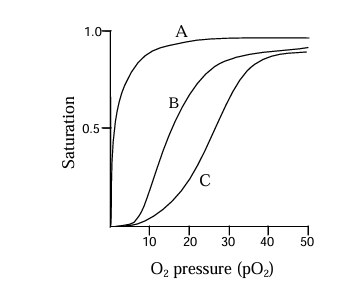
\includegraphics[width=0.7\columnwidth]{FIG/L-17.png}
    \caption*{}
    \label{fig:L-17}
\end{figure}
\begin{enumerate}[label=(\Alph*)]
\item hemoglobin, fetal hemoglobin and myoglobin, respectively
\item fetal hemoglobin, hemoglobin and myoglobin, respectively
\item hemoglobin, myoglobin and fetal hemoglobin, respectively
\item myoglobin, fetal hemoglobin and hemoglobin, respectively
\end{enumerate}

\item A patient comes with symptoms of autonomic hemolysis. The diagnostic tests reveal that he has auto-antibodies to red blood cells (RBCs). Which one of the following mechanisms is the cause of this condition?
\begin{enumerate}[label=(\Alph*)]
\item Neutrophils release granzymes which lyse RBCs
\item Complement is activated and membrane attack complex lyse RBCs
\item Cytotoxic T-cells lyse RBCs
\item Interleukin-2 binds to the receptor on RBCs
\end{enumerate}

\item The nerve impulse at the neuromuscular junction results in discharge of acetylcholine (Ach) from its vesicles into the synaptic cleft. Ach gets degraded by acetylcholine esterase and is present in which one of the following locations?
\begin{multicols}{2}
\begin{enumerate}[label=(\Alph*)]
\item Post synaptic membrane
\item Both pre and post – synaptic clefts
\item Presynaptic membrane
\item Synaptic cleft
\end{enumerate}
\end{multicols}

\item Increasing estradiol (E2) hormone from ovarian follicles prior to ovulation has been hypothesized to play a critical role for induction of pheromones. These pheromones render females sexually receptive to males to facilitate mating. An investigator performs experiments in sheep in which females are gonadectomized, then treated with E2 or vehicle alone and allowed to breed. Which one of the findings listed below will validate the hypothesis that pheromones are induced by E2?
\begin{enumerate}[label=(\Alph*)]
\item Sexual receptivity is regained only in vehicle treated females.
\item Sexual receptivity is regained only in E2 treated females
\item Sexual receptivity was regained irrespective of E2 treatment
\item Sexual receptivity is not regained by any treatment
\end{enumerate}

\end{enumerate}

\begin{center}
\textbf{END OF SECTION - L}
\end{center}
\newpage
\section*{\centering M : FOOD TECHNOLOGY}
\noindent \textbf{ 1 --  10 carry one mark each.}
\begin{enumerate}[label=\arabic*.]

\item Among the following fatty acids, which group is known as essential fatty acids?
\begin{enumerate}[label=(\Alph*)]
\item 9,11-Octadecadienoic and 9,11,13-Octadecatrienoic
\item 9,12-Octadecadienoic and 9,12,15-Octadecatrienoic
\item 9-Octadecenoic and 9,11-Octadecadienoic
\item 9,11-Octadecadienoic and 9-Eicosenoic
\end{enumerate}

\item Cellulose, the structural polysaccharide of plant, is a polymer of
\begin{multicols}{2}
\begin{enumerate}[label=(\Alph*)]
\item $\beta$-D-Glucose
\item $\alpha$-D-Glucose
\item $\beta$-D-Galactose
\item $\alpha$-D-Galcturonic acid
\end{enumerate}
\end{multicols}

\item The important role of carotenoids in the human diet is their ability to serve as precursors of
\begin{multicols}{4}
\begin{enumerate}[label=(\Alph*)]
\item Vitamin C
\item Vitamin D
\item Vitamin A
\item Vitamin K
\end{enumerate}
\end{multicols}

\item Which one of the following microorganisms is used in the preparation of bread?
\begin{multicols}{2}
\begin{enumerate}[label=(\Alph*)]
\item Candida utilis
\item Saccharomyces cerevisiae
\item Saccharomyces cevarum
\item Aspergillus niger
\end{enumerate}
\end{multicols}

\item Which one of the microorganisms given below is NOT RESPONSIBLE for ropy or stringy fermentation of milk?
\begin{multicols}{2}
\begin{enumerate}[label=(\Alph*)]
\item Alcaligenes viscolactis
\item Enterobacter aerogenes
\item Streptococcus cremoris
\item Streptococcus lactis
\end{enumerate}
\end{multicols}

\item A mild heat treatment of foods that destroys pathogens and extends its shelf life is called
\begin{multicols}{4}
\begin{enumerate}[label=(\Alph*)]
\item Baking
\item Blanching
\item Sterilization
\item Pasteurization
\end{enumerate}
\end{multicols}

\item The most common and least expensive plastic film used for packaging of solid food materials is
\begin{multicols}{4}
\begin{enumerate}[label=(\Alph*)]
\item Polyethylene
\item Polystyrene
\item Polypropylene
\item Polyvinylchloride
\end{enumerate}
\end{multicols}

\item Reassociation of amylose and formation of crystalline structure upon cooling of cooked starch solution is termed as
\begin{multicols}{4}
\begin{enumerate}[label=(\Alph*)]
\item Synersis
\item Gelatinization
\item Retrogradation
\item Denaturation
\end{enumerate}
\end{multicols}

\item Thermal destruction of microorganisms follows a kinetics of
\begin{multicols}{4}
\begin{enumerate}[label=(\Alph*)]
\item Zero order
\item First order
\item Second order
\item Fractional order
\end{enumerate}
\end{multicols}

\item 100 kg tomato juice containing 5\% Total Solids (w/w) is concentrated to 25\% Total Solids (w/w). The total amount of water removed from tomato juice in kg is
\begin{multicols}{4}
\begin{enumerate}[label=(\Alph*)]
\item 65
\item 70
\item 75
\item 80
\end{enumerate}
\end{multicols}

\noindent \textbf{ 11 --  20 carry two marks each.}

\item Which one of the following is NOT A CORRECT statement?
\begin{enumerate}[label=(\Alph*)]
\item Meatiness is the taste produced by compounds such as glutamate in products like cheese, soy sauce.
\item Astringency is a dry mouth feel in the oral cavity that is most associated with phenolic compounds.
\item Saltiness is a taste that is mainly produced by chloride ions.
\item Sourness is related to acidity and is sensed by hydrogen ion channels in the human tongue.
\end{enumerate}

\item The following plot represents the Lineweaver-Burk equation of an enzymatic reaction both in the presence and the absence of inhibitor. Here, V is the velocity of reaction and S is the substrate concentration.

\begin{figure}[H]
    \centering
    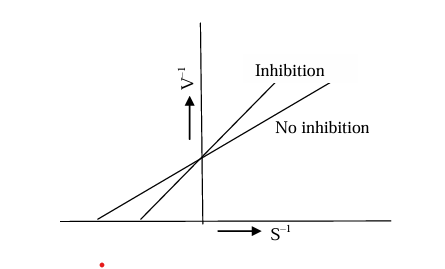
\includegraphics[width=0.7\columnwidth]{FIG/M-12.png}
    \caption*{}
    \label{fig:M-12}
\end{figure}

The nature of inhibition shown in the plot is
\begin{multicols}{2}
\begin{enumerate}[label=(\Alph*)]
\item Non-competitive
\item Anti-competitive
\item Competitive
\item Mixed type
\end{enumerate}
\end{multicols}

\item Make the correct match of the food constituents in Group I with their nature given in Group II.
\begin{center}
\begin{tabular}{p{6cm} p{6cm}}
\textbf{Group I} & \textbf{Group II} \\
P) Ascorbic Acid & 1) Sugar \\
Q) Phenyl alanine & 2) Chelate \\
R) Dextrose & 3) Amino Acid \\
S) Haemoglobin & 4) Antioxidant \\
\end{tabular}
\end{center}
\begin{multicols}{2}
\begin{enumerate}[label=(\Alph*)]
\item P-4, Q-3, R-1, S-2
\item P-4, Q-1, R-3, S-2
\item P-3, Q-4, R-2, S-1
\item P-4, Q-2, R-1, S-3
\end{enumerate}
\end{multicols}

\item Make the correct match of the fermented food products in Group I with the microorganisms in Group II.
\begin{center}
\begin{tabular}{p{6cm} p{6cm}}
\textbf{Group I} & \textbf{Group II} \\
P) Yoghurt & 1) Lactobacillus acidophilus and Lactobacillus delbrueckii \\
Q) Cheese & 2) Leuconostoc mesenteroides and Lactobacillus plantarum \\
R) Sauerkraut & 3) Lactobacillus delbrueckii and Streptococcus thermophillus \\
S) Kefir & 4) Lactobacillus casei and Streptococcus thermophillus \\
\end{tabular}
\end{center}
\begin{multicols}{2}
\begin{enumerate}[label=(\Alph*)]
\item P-1, Q-4, R-2, S-3
\item P-4, Q-3, R-1, S-2
\item P-3, Q-4, R-2, S-1
\item P-3, Q-2, R-4, S-1
\end{enumerate}
\end{multicols}

\item Match the following between organelle or cellular components of a bacterium cell in Group I with the constituents and functionalities in Group II.
\begin{center}
\begin{tabular}{p{6cm} p{6cm}}
\textbf{Group I} & \textbf{Group II} \\
P) Cytoplasmic membrane & 1) Protein synthesis \\
Q) Flagellum & 2) Peptidoglycan \\
R) Cell wall & 3) Phospholipid bilayer \\
S) Ribosome & 4) Motility of cell \\
\end{tabular}
\end{center}
\begin{multicols}{2}
\begin{enumerate}[label=(\Alph*)]
\item P-3, Q-2, R-4, S-1
\item P-4, Q-2, R-1, S-3
\item P-3, Q-4, R-2, S-1
\item P-2, Q-3, R-4, S-1
\end{enumerate}
\end{multicols}

\item Thermal death time (TDT) of \textit{Clostridium botulinum} at 121$^\circ$C is 2.78 min with a z-value of 10$^\circ$C. The TDT of the microorganism at 116$^\circ$C (in min) is
\begin{multicols}{4}
\begin{enumerate}[label=(\Alph*)]
\item 5.270
\item 8.791
\item 1.390
\item 0.712
\end{enumerate}
\end{multicols}

\item Make the correct match between specific food processing operations in Group I with their mechanism of action in Group II.
\begin{center}
\begin{tabular}{p{6cm} p{6cm}}
\textbf{Group I} & \textbf{Group II} \\
P) Ball Mill & 1) Compression and shear \\
Q) Roller Mill & 2) Pressure bursting \\
R) Flash Peeling & 3) Friction and shear \\
S) Abrasive Peeling & 4) Impact and shear \\
\end{tabular}
\end{center}
\begin{multicols}{2}
\begin{enumerate}[label=(\Alph*)]
\item P-4, Q-2, R-1, S-3
\item P-4, Q-1, R-2, S-3
\item P-4, Q-3, R-2, S-1
\item P-3, Q-1, R-4, S-2
\end{enumerate}
\end{multicols}

\item 650 g of a wet food containing 405 g water is dried in a tray dryer to a final moisture content of 6.8\% (dry basis). It is observed that the drying process occurs under constant rate period and it takes 8 h. The rate of drying (in kg/h) is
\begin{multicols}{4}
\begin{enumerate}[label=(\Alph*)]
\item 128.79
\item 126.35
\item 77.81
\item 0.0485
\end{enumerate}
\end{multicols}

\item Air at 1 atmospheric pressure (101.325 kPa) and 30$^\circ$C with absolute humidity of 0.0218 kg/kg of dry air is flowing in a drying chamber. The saturated vapor pressure of water ($p_w^0$, in kPa) is related to temperature ($T$, in $^{\circ}C$) as given below:
\[
\ln p_w^0 =  5217.635 / (T + 273) - 18.6556
\]
The relative humidity of air (in percentage) is
\begin{multicols}{4}
\begin{enumerate}[label=(\Alph*)]
\item 62.82
\item 68.22
\item 86.62
\item 81.80
\end{enumerate}
\end{multicols}

\item The total solids content in a milk sample is 18 \%. It is desired to produce 1000 kg of sweetened condensed milk (SCM) having 40 \% sugar, 25 \% moisture and rest milk solids. What is the ‘Sugar Ratio’ (in percentage) in the SCM in terms of sugar and water content in the final product?
\begin{multicols}{4}
\begin{enumerate}[label=(\Alph*)]
\item 48.19
\item 61.54
\item 54.16
\item 56.14
\end{enumerate}
\end{multicols}

\end{enumerate}

\begin{center}
\textbf{END OF QUESTION PAPER}
\end{center}

\end{document}

